% Created 2012-05-25 Fri 12:20
\documentclass[compress, 9pt]{beamer}
\usepackage[utf8]{inputenc}
\usepackage[T1]{fontenc}
\usepackage{fixltx2e}
\usepackage{graphicx}
\usepackage{longtable}
\usepackage{float}
\usepackage{wrapfig}
\usepackage{soul}
\usepackage{textcomp}
\usepackage{marvosym}
\usepackage{wasysym}
\usepackage{latexsym}
\usepackage{amssymb}
\tolerance=1000
\usetheme{default}
\usecolortheme[RGB={0,38,93}]{structure}
\usefonttheme{serif}
\useinnertheme{circles}
\useoutertheme[]{shadow}
\setbeamertemplate{navigation symbols}{}
\usepackage{natbib}
\usepackage{fleqn}
\usepackage{epsf}
\usepackage[dvips]{color}
\usepackage{bibentry}
\institute{Computer Science and Engineering \\ University of Michigan}
\providecommand{\alert}[1]{\textbf{#1}}

\title{Classical Planning}
\author{Shiwali Mohan}
\date{\today}
\hypersetup{
  pdfkeywords={},
  pdfsubject={},
  pdfcreator={Emacs Org-mode version 7.8.09}}

\begin{document}

\maketitle

\begin{frame}
\frametitle{Outline}
\setcounter{tocdepth}{3}
\tableofcontents
\end{frame}


\title[Search \hspace{1em}\insertframenumber/
\inserttotalframenumber]{Full Title}

\section{Classical Planning}
\label{sec-1}
\begin{frame}
\frametitle{Review}
\label{sec-1-1}
\begin{itemize}

\item <1-> What is a plannning problem?
\label{sec-1-1-1}%
\begin{itemize}
\item <2-> asks if we can reach a goal state from the initial state
\item <2-> how?
\end{itemize}

\item <3-> Environment is
\label{sec-1-1-2}%
\begin{itemize}
\item <3-> fully observable
\item <3-> deterministic
\item <3-> finite
\item <3-> static
\item <3-> discrete
\end{itemize}

\item <4-> Combination of
\label{sec-1-1-3}%
\begin{itemize}
\item <4-> Logic (state and action representation)
\item <4-> Search (search for generating a plan)
\end{itemize}

\item <5-> State Representation
\label{sec-1-1-4}%
\begin{itemize}
\item <6-> Conjunction of ground, functionless terms (fluents)
\begin{itemize}
\item examples: Poor \^{} Unknown; At(Truck1, Melbourne)
\end{itemize}
\item <6-> Close world assumption
\begin{itemize}
\item <7-> fluents that are not mentioned are false
\item <7-> objects with unique names are distinct
\end{itemize}
\item <8-> \texttt{at(Truck1,y)?}, \texttt{-Wealthy?}, \texttt{At(Father(Fred),Sydney)},
  \texttt{On(blockA, blockB) V On (blockA, blockC)}
\end{itemize}
\end{itemize} % ends low level
\end{frame}
\begin{frame}[fragile]
\frametitle{Review}
\label{sec-1-2}
\begin{itemize}

\item Action Representation
\label{sec-1-2-1}%
\begin{itemize}
\item as action schemas
\item single schema represents a set of ground actions
\end{itemize}
\begin{verbatim}
     Action(Fly(p, from, to),
        PRECOND: At(p,from) ^ Plane (p) ^ Airport (from) 
                 ^ Airport (to)
        EFFECT: -At(p,from) ^ At(p,to))
\end{verbatim}
\begin{itemize}
\item Universally quantified
\item applicable in states where all the preconditions are satisfied
\item delete list: remove fluents that appear as negative literals in effects
\item add list: add fluents that appear as positive literals in effects
\end{itemize}

\end{itemize} % ends low level
\end{frame}
\section{PDDL}
\label{sec-2}
\begin{frame}
\frametitle{PDDL Formulation}
\label{sec-2-1}
\begin{columns}
\begin{column}{0.5\textwidth}
%% questions
\label{sec-2-1-1}

\begin{itemize}
\item <1-> What predicates would you use to represent the problem?
\begin{itemize}
\item <2-> \texttt{clear(), on(), smaller(), disk()}
\end{itemize}
\item <3-> What is the initial state?
\begin{itemize}
\item <4-> \texttt{on(Red, Green), on(Green, Blue)},
         \texttt{on(Blue, A), clear(Red), disc(Red) ...}
         \texttt{clear(B), clear(C), smaller(Red, Green)} 
         \texttt{smaller(Red, Blue), smaller(Red, A)} \ldots{}
\end{itemize}
\item <5-> What is the goal state?
\begin{itemize}
\item <6-> \texttt{on(Red, Green), on(Green, Blue), on(Blue, C)}
\end{itemize}
\end{itemize}
\end{column}
\begin{column}{0.5\textwidth}
%% toh
\label{sec-2-1-2}

 \begin{figure}[htb]
 \centering
 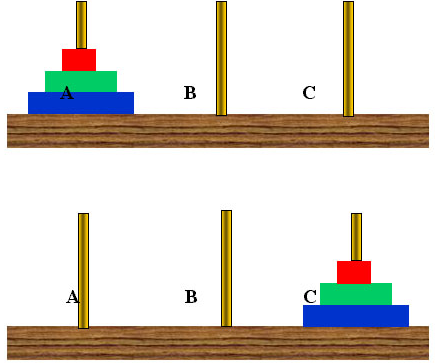
\includegraphics[width=5cm]{../images/torrehanoi.png}
 \caption{objects: disks - red, green, blue; pegs - A, B, C}
 \end{figure}
\end{column}
\end{columns}
%% actions
\label{sec-2-1-3}

\begin{itemize}
\item <7-> How are actions defined?
\begin{itemize}
\item <8-> \texttt{Action(move(disk, source, destination)}\\
\texttt{PRECOND: clear(disk) \textasciicircum{} on(disk, source) \textasciicircum{} clear(destination)     \textasciicircum{}smaller(disk,destination)}\\
             \texttt{EFFECT: on(disk, destination) \textasciicircum{} -on(disk, source) \textasciicircum{} -clear(destination) \textasciicircum{}clear(source)}
\end{itemize}
\end{itemize}
\end{frame}
\section{Planning Graph}
\label{sec-3}
\begin{frame}
\frametitle{Planning Graph Review}
\label{sec-3-1}
\begin{itemize}

\item <1-> Directed graph
\label{sec-3-1-1}%
\begin{itemize}
\item <1-> organized into levels
\item <1-> level $S_0$ is the initial state that consists of fluents that hold
  in $S_0$
\item <1-> level $A_0$ consisting of actions applicable in $S_0$.
\item <1-> Alternate $S_i$ and $A_i$ until termination
\item <1-> persistence actions and mutex
\end{itemize}
\end{itemize} % ends low level
%% <2-> image
\label{sec-3-1-2}

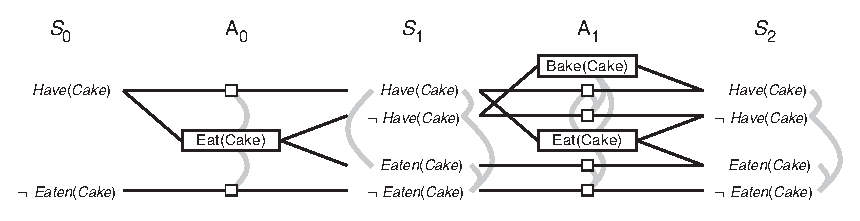
\includegraphics[width=10cm]{../images/eatcake-graphplan2.eps}
\begin{itemize}

\item Uses
\label{sec-3-1-3}%
\begin{itemize}
\item for generating plans
\item for heuristic estimation
\end{itemize}
\end{itemize} % ends low level
\end{frame}
\begin{frame}[fragile]
\frametitle{Spare Tire Example (in book)}
\label{sec-3-2}


\begin{verbatim}
Init(Tire(Flat) ^ Tire(Spare) ^ At(Flat,Axle) ^ at(Spare,Trunk))
Goal(At(Spare,Axle))
Action(Remove(obj,loc),
    PRECOND: At(obj,loc)
    EFFECT: -At(obj,loc) ^ At(obj,ground))
Action(PutOn(t,Axle),
    PRECOND: Tire(t) ^ At(t,Ground) ^ -At(Flat,Axle)
    EFFECT: -At(t,Ground) ^ At(t,Axle)
Action(LeaveOvernight)
    PRECOND:
    EFFECT: -At(Spare,Ground) ^ -At(Spare,Axle) ^ -At(Spare,Trunk) 
            ^-At(Flat,Ground) ^ -At(Flat,Axle) ^-At(Flat,Trunk)
\end{verbatim}
\end{frame}
\begin{frame}
\frametitle{Spare Tire Example (in book)}
\label{sec-3-3}

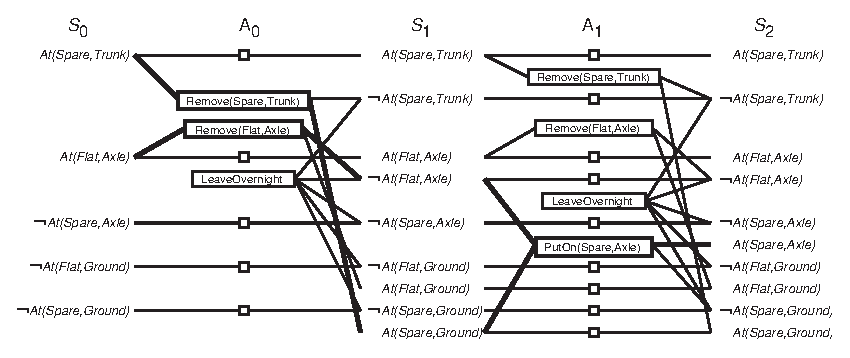
\includegraphics[width=10cm]{../images/tire-graphplan2-no-mutex.eps}
\begin{itemize}
\item <1-> Mutex actions?
\begin{itemize}
\item <2-> Inconsistent effects?
\begin{itemize}
\item <3-> one action negates an effect of the other
\item <8-> \texttt{Remove(Spare,Trunk)} with \texttt{LeaveOvernight}
\end{itemize}
\item <4-> Interference?
\begin{itemize}
\item <5-> one of the effects of an action is the negation of a
      precondition of the other
\item <8-> \texttt{Remove(Flat,Axle)} with \texttt{LeaveOvernight}
\end{itemize}
\item <6-> Competing needs?
\begin{itemize}
\item <7-> One of the preconditions of one action is mutually
      exclusive with a precondition of the other
\item <8-> \texttt{PutOn(Spare,Axle)} with \texttt{Remove(Flat,Axle)}
\end{itemize}
\end{itemize}
\end{itemize}
\end{frame}
\begin{frame}
\frametitle{Spare Tire Example (in book)}
\label{sec-3-4}

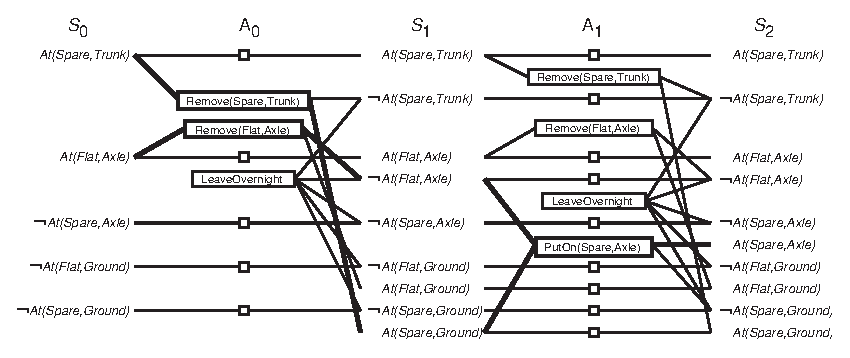
\includegraphics[width=10cm]{../images/tire-graphplan2-no-mutex.eps}
\begin{itemize}
\item <1-> Mutex literals?
\begin{itemize}
\item <1-> Negated literal?
\item <2-> Inconsistent support?
\begin{itemize}
\item <3-> if each possible pair of actions that achieve the two
      literal is mutex
\item <4-> \texttt{At(Spare, Axle)} with \texttt{At(Flat,Axle)} in S2
\end{itemize}
\end{itemize}
\end{itemize}
\end{frame}
\begin{frame}
\frametitle{Extract Solution}
\label{sec-3-5}

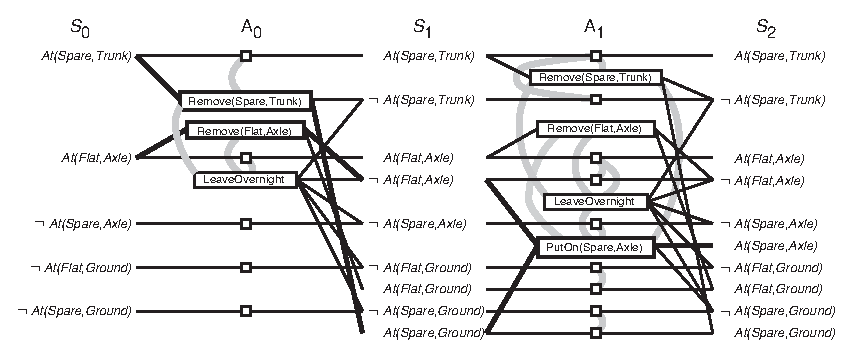
\includegraphics[width=10cm]{../images/tire-graphplan2.eps}
\begin{itemize}

\item Extract Solution can be formulated as CSP or backward search
\label{sec-3-5-1}%

\item As a CSP
\label{sec-3-5-2}%
\begin{itemize}
\item variables? values?
\item constraints?
\end{itemize}

\item As backward search
\label{sec-3-5-3}%
\begin{itemize}
\item Initial state?
\item Goal?
\item Actions?
\item Cost
\end{itemize}

\end{itemize} % ends low level
\end{frame}

\end{document}
